\documentclass[11pt]{article}
\usepackage{graphicx}
\begin{document}

\title{Automated Music Generation}

\author{Suyash Kumar}

\maketitle

\section{Aim}
The aim of the project is to create a machine learning model that is able to generate {\em original} music after being trained on several music pieces.
\section{Introduction}
This project attempts to tackle this problem by using a class of neural networks called "Recurrent Neural Networks". This class of neural networks is distinguished from others due to the fact that they are {\bf able to model memory}. This is especially important while working on sequential data.

Traditional neural networks consist of an input layer, a series of hidden layer and the output layer. The hidden layer takes as input only the outputs of the input layer. However, in recurrent neural networks, the hidden layer is a function of the input layer as well as the previous representation of the hidden layer, creating a feedback loop. This feedback loop is able to model memory, and is representative of all the inputs that have been seen so far. Such a network is then able to work for sequential data. Music is represented as sequential data, the data is represented as chords that are played in sequence at various timestamps.

Recurrent Neural Networks(RNNs), Long Short Term Memory Networks(LSTMs) and Generative Adversarial Networks are some of the types of networks/approaches that have been tried out in this attempt.
%\section{History}
%Historically, there have been many approaches to tackling the task of computationally %generating music. 
\section{Background}
\subsection{Recurrent Neural Networks}
Recurrent Neural Networks are neural networks in which neurons form a directed cycle. This creates an internal state that is able to exhibit temporal behavior, and can be used to process sequential data such as images, written information, or in this case, music.

RNNs have a memory associated with it which can capture information about the inputs witnessed so far. Theoretically, RNNs should be able to process arbitrarily long sequences, however in practice, they can only look back a few steps.

\begin{figure}
  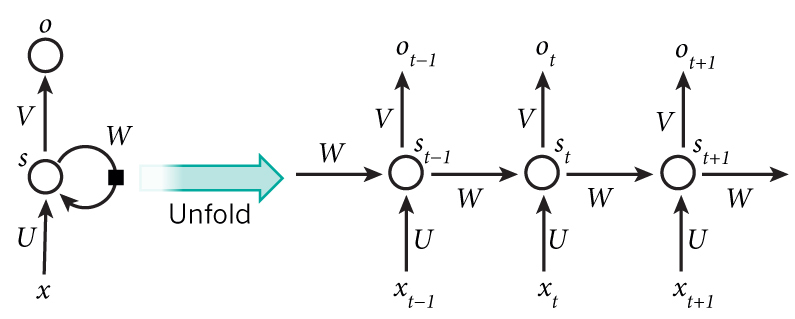
\includegraphics[width=\linewidth]{rnn.jpg}
  \caption{Representation of an RNN, and unfolding the network}
  \label{fig:rnn}
\end{figure}

As can be seen in the figure, the hidden layers have an edge to itself, meaning the hidden layer takes inputs from the input layer and the hidden layer from the previous timestep. It is equivalent to the unrolled neural network as shown in the figure.

In the figure, xt is the input at time step t. st is the hidden state at step t. st is calculated as follows:

st = f(Uxt + Wst-1)

where U, V, W are the corresponding weights as shown in the figure.

The function f is an activation function like tanh. ot is the output at step t.

The neural network uses the backpropagation through time algorithm for learning the weights U,V and W.

\subsection{Long Short Term Memory Networks}

RNNs generally have difficulties in learning long-range sequential data. This is often attributed to the \emph{Vanishing Gradient problem}, which arises because of the chosen activation function(tanh). The deriviatives of tanh function are in the range (-1,1), and 

\subsection{Generative Adversarial Networks}
\section{Model}
\subsection{ABC notation}
The initial recurrent neural network uses abc notation as input. ABC notation is a shorthand form of musical notation. In basic form it uses the letters A through G to represent the given notes, with other elements used to place added value on these - sharp, flat, the length of the note, key, ornamentation. Since ABC notation is in essence a textual data, a character level recurrent neural network, which takes as input individual characters at a time can be created.

The dataset comprises of 1000 tunes scraped from The Nottingham Music database : http://ifdo.ca/~seymour/nottingham/nottingham.html. The abc notation of each tune was concatenated to get a single training data file.

abc2midi program has been used to convert the generated abc notation to midi files. timidity program has been used to play these midi files.

\subsection{Character Level Model}
A recurrent neural network, whose input and output consists of only a single character is called a character level model. Following this representation, a recurrent neural network may be created for virtually any kind of textual data. Historically, similar models have been tried out for various kind of data sets, such as -
\begin{itemize}
\item Shakespeare's Plays
\item Wikipedia Articles
\item HTML documents
\item LATEX documents
\item C++ code
\item Research Papers
\item Music
\end{itemize}

These models were able to generate documents that \emph{looked} similar to the training documents, however sometimes the network wasn't able to capture subtleties like the grammar/format involved with a particular type of document.

\subsection{Music Generation Model}


\section{Results and Analysis}
\section{Conclusion}
\section{Bibliography}
\end{document}